\documentclass[12pt,a4paper]{article}
\usepackage[utf8]{inputenc}
\usepackage{amssymb, amsmath, multicol}
\usepackage[russian]{babel}
\usepackage{graphicx}
\usepackage[shortcuts,cyremdash]{extdash}
\usepackage{wrapfig}
\usepackage{floatflt}
\usepackage{lipsum}
\usepackage{concmath}
\usepackage{euler}
\usepackage{tikz}  
\usetikzlibrary{graphs}

\oddsidemargin=-15.4mm
\textwidth=190mm
\headheight=-32.4mm     
\textheight=277mm
\tolerance=100
\parindent=0pt
\parskip=8pt
\pagestyle{empty}
\renewcommand{\tg}{\mathop{\mathrm{tg}}\nolimits}
\renewcommand{\ctg}{\mathop{\mathrm{ctg}}\nolimits}
\renewcommand{\arctan}{\mathop{\mathrm{arctg}}\nolimits}
\newcommand{\divisible}{\mathop{\raisebox{-2pt}{\vdots}}}

\graphicspath{{pictures/}}

\begin{document}
	\begin{center}
		Работа 2.1.3 \\
		
		"Определение $C_p / C_v$ по скорости звука в газе" \\
		
		Б01-005 Радькин Кирилл
	\end{center}
	
	Цель работы:
	
	\begin{itemize}
		\item Измерение частоты колебаний и длины волны при резонансе звуковых колебаний в газе, заполняющем трубу	
		
		\item Определение показателя адиабаты с помощью уравнения состояния идеального газа	
	\end{itemize}
	
	В работе используются: 
	\begin{itemize}
		\item Звуковой генератор ГЗ; электронный осциллограф ЭО; микрофон; телефон; раздвижная труба; тепло- изолированная труба, обогреваемая водой из термостата; баллон со сжатым углекислым газом; газгольдер.
	\end{itemize}
	
	Скорость распространения звуковой волны в газах зависит от показателя адиабаты $\gamma$. На измерении скорости звука основан один из наиболее точных методов определения показателя адиабаты. \\
	
	Скорость звука в газах определяется формулой:
	
	\begin{equation*}
		c = \sqrt{\gamma \dfrac{RT}{\mu}}
	\end{equation*}
	
	где $R$ — газовая постоянная, $T$ — температура газа, а $\mu$ — его молярная масса. Преобразуя эту формулу, найдем:
	
	\begin{equation}
		\gamma = \dfrac{\mu}{RT} c^2
	\end{equation}
	
	Таким образом, для определения показателя адиабаты достаточно измерить температуру газа и скорость распространения звука (молярная масса газа предполагается известной).\\
	
	Звуковая волна, распространяющаяся вдоль трубы, испытывает многократные отражения от торцов. Звуковые колебания в трубе являются наложением всех отраженных волн и, вообще говоря, очень сложны. Картина упрощается, если длина трубы $L$ равна целому числу полуволн, то есть когда:
	
	\begin{equation}
		L = \dfrac{n \lambda}{2}
	\end{equation}
	
	где $\lambda$ — длина волны звука в трубе, а $n$ — любое целое число. Если условие (2) выполнено, то волна, отраженная от торца трубы, вернувшаяся к ее началу и вновь отраженная, совпадает по фазе с падающей. Совпадающие по фазе волны усиливают друг друга. Амплитуда звуковых колебаний при этом резко возрастает — наступает резонанс.\\
	
	При звуковых колебаниях слои газа, прилегающие к торцам трубы, не испытывают смещения (узел смещения). Узлы смещения повторяются по всей длине трубы через $\dfrac{\lambda}{2}$. Между узлами находятся максимумы смещения (пучности).\\
	
	Скорость звука c связана с его частотой $f$ и длиной волны $\lambda$ соотношением:
	
	\begin{equation}
		c = \lambda f
	\end{equation}
	
	Подбор условий, при которых возникает резонанс, можно производить двояко:
	\begin{enumerate}
		\item При неизменной частоте $f$ звукового генератора (а следовательно, и неизменной длине звуковой волны $\lambda$) можно изменять длину трубы $L$. Для этого применяется раздвижная труба. Длина раздвижной трубы постепенно увеличивается, и наблюдается ряд последовательных резонансов. Возникновение резонанса легко наблюдать на осциллографе по резкому увеличению амплитуды колебаний. Для последовательных резонансов имеем:
		
		\begin{equation*}
			L_n = n\dfrac{\lambda}{2}, L_{n+1} = (n + 1)\dfrac{\lambda}{2}, \cdots, L_{n+k} = n\dfrac{\lambda}{2} + k\dfrac{\lambda}{2}
		\end{equation*}
		
		т. е. $\dfrac{\lambda}{2}$ равно угловому коэффициенту графика, изображающего зависимость длины трубы $L$ от номера резонанса $k$. Скорость звука находится по формуле (3).
		\item При постоянной длине трубы можно изменять частоту звуковых колебаний. В этом случае следует плавно изменять частоту $f$ звукового генератора, а следовательно, и длину звуковой волны $\lambda$.\\
		
	Для последовательных резонансов получим:
	
	\begin{equation}
		L = \dfrac{\lambda_1}{2}n = \dfrac{\lambda_2}{2}(n+1) = \cdots = \dfrac{\lambda_{k+1}}{2}(n+k)
	\end{equation}
	
	Из (3) и (4) имеем:
	
	\begin{equation}
		f_1 = \dfrac{c}{\lambda_1} = \dfrac{c}{2L}n, f_2 = \dfrac{c}{\lambda_2}=\dfrac{c}{2L}(n+1)=f_1 + \dfrac{c}{2L}, \cdots f_{k+1} = \dfrac{c}{\lambda_{k+1}} = \dfrac{c}{2L}(n+k) = \dfrac{c}{2L}k + f_1		
	\end{equation}
	
	Скорость звука, деленная на $2L$, определяется, таким образом, по угловому коэффициенту графика зависимости частоты от номера резонанса.
	\end{enumerate}
	
	Экспериментальная установка:\\
	
	Соответственно двум методам измерения скорости звука в работе имеются две установки (рис. 1 и 2). В обеих установках звуковые колебания в трубе возбуждаются телефоном Т и улавливаются микрофоном М. Мембрана телефона приводится в движение переменным током звуковой частоты; в качестве источника переменной ЭДС используется звуковой генератор ГЗ. Возникающий в микрофоне сигнал наблюдается на осциллографе ЭО.\\
	
	Микрофон и телефон присоединены к установке через тонкие резиновые трубки. Такая связь достаточна для возбуждения и обнаружения звуковых колебаний в трубе и в то же время мало возмущает эти колебания: при расчетах оба торца трубы можно считать неподвижными, а влиянием соединительных отверстий пренебречь.\\
	
	\begin{center}
		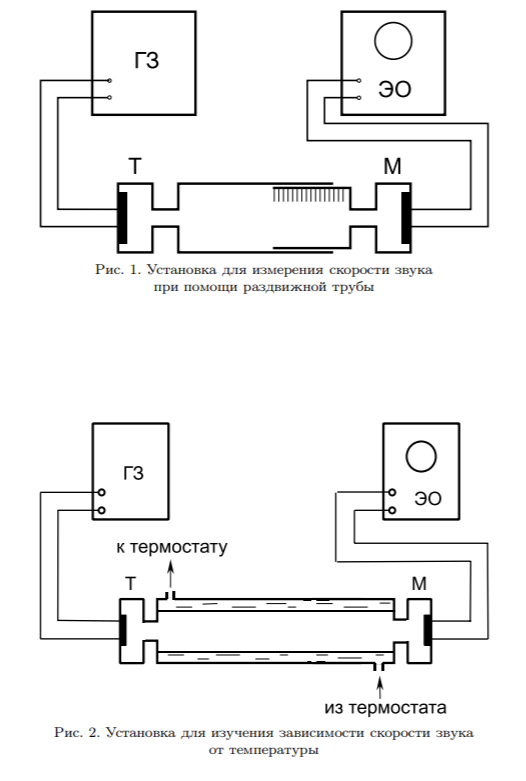
\includegraphics[scale=1]{pic1.png}
	\end{center}
	
	Первая установка (рис. 1) содержит раздвижную трубу с миллиметровой шкалой. Через патрубок (на рисунке не показан) труба может наполняться воздухом или углекислым газом из газгольдера. На этой установке производятся измерения $\gamma$ для воздуха и для $CO_2$ .\\
	
	Вторая установка (рис. 2) содержит теплоизолированную трубу постоянной длины. Воздух в трубе нагревается водой из термостата. Температура газа принимается равной температуре омывающей трубу воды. На этой установке измеряется зависимость скорости звука от температуры.\\
	
	\begin{center}
		Ход работы:
	\end{center}
	
	\begin{enumerate}
		\item Включим в сеть электронный осциллограф ЭО и звуковой генератор ГЗ и дадим им прогреться 5–7 минут. После этого включим тумблер «Луч» и ручками управления осциллографа добъемся того, чтобы на экране была видна линия, прочерченная электронным лучом.\\
		
	Установим нулевое значение шкалы частот звукового генератора (только для генератора ГЗ-18). Для этого лимбы «Частота» и «Расстройка» установим на нуль и вращением ручки «Установка нуля» добъемся того, чтобы стрелка вольтметра остановилась на нуле. Время от времени проверяем, не сбилась ли установка нуля.
	
	\item Подберем напряжение на выходе генератора так, чтобы при резонансе на осциллографе наблюдались колебания достаточной амплитуды. Остановим картину на осциллографе. Убедитесь в том, что колебания имеют неискаженную синусоидальную форму. Если форма колебаний искажена, уменьшаем амплитуду сигнала, поступающего с генератора, пока искажения не прекратятся.
	
	\item Измерения на первой установке (рис. 1):
	
		\begin{enumerate}
			\item Исходя из примерного значения скорости звука (300 м/с), рассчитаем, в каком диапазоне частот следует вести измерения, чтобы при удлинении трубы можно было наблюдать 2–5 резонансов.\\
			
			Диапазон изменение длины трубы: $\Delta l = 230$ мм $\rightarrow$ в него должно укладываться 5 полуволн $\rightarrow$ $\lambda \leqslant 0.115$ м $\rightarrow f \geqslant 2600$ Гц
			\item Используя многоходовый или кнопочный кран, продуем трубу воздухом (в ней мог остаться углекислый газ). Плавно изменяя длину трубы, последовательно пройдем через все доступные для наблюдения точки резонанса. Повторим измерения при других частотах (всего 4–6 различных значений частоты). Для каждого резонанса измерим соответствующее удлинение трубы. Проведем измерения, сначала увеличивая длину трубы, а затем уменьшая ее.(вернхняя строка таблицы~---~при уменьшении, нижняя~---~при увеличении).\\
			
		\begin{tabular}{|c|c|c|c|c} \hline
			\multicolumn{5}{|c|}{$L, $мм} \\ \hline
			\multicolumn{5}{|c|}{$f = 2021$ Гц} \\ \hline
			32 & 118 & 202 \\ \hline
			28 & 116 & 197 \\ \hline
			\multicolumn{5}{|c|}{$f = 2506$ Гц} \\ \hline	
		\end{tabular}
		\end{enumerate}
	\end{enumerate}
\end{document}